\documentclass[a4paper, 12pt]{report}
\usepackage[utf8]{inputenc}
\usepackage[T2A]{fontenc}
\usepackage[english,russian]{babel}
\usepackage[dvips]{graphicx}
\usepackage[left = 2cm, top = 1cm, right = 2cm, bottom = 2cm]{geometry}
\usepackage{hyperref}
\usepackage{xcolor}
\usepackage{titlesec}
\usepackage{listings}
\usepackage{amsthm}
\usepackage{amsmath}
\usepackage{eufrak}

\usepackage{color}

\newtheorem*{definition}{Определение}

\lstloadlanguages{C,[ANSI]C++}%,Clean,make,Fortran}%Загружаемые языки
\lstset{extendedchars=false,
        breaklines=true, %автоперенос длинных линий
        breakatwhitespace=true}
\graphicspath{{pic/}}
\titleformat{\chapter}[block]{\color{black}\Large\bfseries\filcenter}{}{1em}{}
\setcounter{secnumdepth}{0}

\begin{document}
\title{Основания алгебраического подхода к синтезу корректных алгоритмов}
\author{Лектор --- Рудаков К.В.\\ Наборщик --- Старожилец В.М.}
\date{}
\maketitle

\tableofcontents

\chapter{Лекция 1}
\section{Введение}
Данные лекции рассматривают общую задачу машинного обучения без привязки к конкретным методам и основы алгебраического подхода к синтезу корректных алгоритмов для её решения. В некотором роде они являются взглядом сверху на задачи машинного обучения и методы их решения.

В первую очередь следует сформулировать задачу машинного обучения в общем виде. По сути это задача построения алгоритма, который реализует отображение из множества начальных информаций в множество конечных информаций. Сразу отметим, что в курсе рассматриваются только такие отображения, для которых существует реализующий их алгоритм.

\begin{definition}
Символом $\mathfrak{I_i}$ (читается <<И инишл>>) будем обозначать множество начальных информаций, например, симптомы болезни.
\end{definition}

\begin{definition}
Символом $\mathfrak{I_f}$ (читается <<И файнэл>>) будем обозначать множество конечных информаций, например, диагноз.
\end{definition}

Таким образом, на формальном языке нам требуется найти такой алгоритм $A$, что он осуществляет отображение из множества начальных информаций $\mathfrak{I_i}$ в множество конечных информаций $\mathfrak{I_f}$:
\[
A: \mathfrak{I_i} \rightarrow \mathfrak{I_f}.
\]
Пока что задача стоит так, что нам нужно найти некоторое произвольное отображение из одного множества в другое, реализуемое некоторым алгоритмом. При этом свойства этого отображения и алгоритма неважны. В такой постановке у нас нет каких-либо ограничений на искомый алгоритм: даже датчик случайных чисел является решением этой задачу. Поэтому вводятся дополнительные ограничения на допустимые алгоритмы. Итак,

\begin{definition}
Обозначим $\mathfrak{M}^* = \{A|\ A:\  \mathfrak{I_i}\rightarrow \mathfrak{I_f}\}$ множество всех алгоритмов, реализующих отображение из $\mathfrak{I_i}$ в $\mathfrak{I_f}$.
\end{definition}

\begin{definition}
Обозначим $I_{str}$ структурную информацию, содержащую условия и требования, накладываемые на $A$.
\end{definition}

\begin{definition}
Обозначим $\mathfrak{M}(I_{str}) \subset \mathfrak{M}^*$ некоторое подмножество $\mathfrak{M}^*$, удовлетворяющее $I_{str}$.
\end{definition}

Теперь у нас есть дополнительная информация $I_{str}$, позволяющий накладывать дополнительные ограничения на нашу задачу. Введём определения допустимого отображения и корректного алгоритма.

\begin{definition}
Любое отображение из множества $\mathfrak{M}(I_{str})$ называется допустимым.
\end{definition}

\begin{definition}
Задача Z заключается в построении алгоритма, реализующего допустимое отображение.
\end{definition}

\begin{definition}
Любой алгоритм реализующий любое допустимое отображение называется корректным.
\end{definition}

В такой формулировке необходимым и достаточным условием разрешимости задачи Z является выполнение выражения: \[
\mathfrak{M}(I_{str}) \neq \emptyset,
\]
а условием единственности решения~--- выполнение равенства:
\[
|\mathfrak{M}(I_{str})| = 1.
\]
Заметим также, что в данной формулировке корректный алгоритм~--- это алгоритм, не допускающий ни одной ошибки, а множество $\mathfrak{M}(I_{str})$~--- множество алгоритмов не допускающих ошибок. Однако можно поставить условия несколько мягче, и дать алгоритмам возможность ошибаться.

\section{Поиск решения задачи}
Пусть $\mathfrak{M}(\pi)$~--- некоторое параметрическое семейство отображений. После того как мы выбрали некоторое семейство отображений $\mathfrak{M}(\pi)$, попытаемся попасть в $\mathfrak{M}(I_{str})$, взяв в $\mathfrak{M}(\pi)$ какое-нибудь отображение за начальное. Это возможно, если данные семейства пересекаются:
\[
\mathfrak{M}(\pi) \cap \mathfrak{M}(I_{str}) \neq \emptyset.
\]

Но, с одной стороны, чем \emph{сложнее} наше семейство, тем выше вероятность, что оно пересекается с семейством $\mathfrak{M}(I_{str})$, однако, с другой стороны, достижение этого пересечения может быть \emph{затратно}, если $\mathfrak{M}(\pi)$ сложное. Также всегда остаётся вероятность, что множество $\mathfrak{M}(\pi)$ с $\mathfrak{M}(I_{str})$ не пересекается. Для поиска компромиссного решения используют идею \emph{расширения множества}.

\begin{definition}
Пусть $f$~--- некоторая операция над множеством $\mathfrak{M}^*$. Тогда $f(\mathfrak{M}(\pi))$ будем называть расширением множества $\mathfrak{M}(\pi)$.
\end{definition}

Таким образом, мы хотим расширить некоторое <<простое>> множество до пересечения с $\mathfrak{M}(I_{str})$. Однако, не любая функция $f$ нам подходит, так как <<простое>> множество может расшириться до слишком <<сложного>> множества. Важно, что $f$ мы выбираем сами, поэтому можем выбрать его так, чтобы искать нужный алгоритм было не слишком сложно.

\chapter{Лекция 2}
\section{Алгебра, реляционная система и алгебраическая система}
Данная лекция скорее просвещена вопросам терминологии в данном курсе. Поэтому, тут будет очень много определений (ещё больше, чем в предыдущей). Для начала определим понятия алгебры, реляционной системы и алгебраической системы.

\begin{definition}
Сигнатура~---набор характеристик, однозначно идентифицирующий объект.
\end{definition}

\begin{definition}
Отношение~—-- математическая структура, которая формально определяет свойства различных объектов и их взаимосвязи. В нашем курсе будет обозначаться буквой $R$.
\end{definition} 

\begin{definition}
Алгеброй называется структура
\[
\left(
\begin{array}{ccccc}
  A & Op_1 & Op_2 & ... & Op_k \\
    & n_1 & n_2 & ... & n_k 
\end{array}
\right)
\]
где A~--- множество, $Op_i$~--- операции на этом множестве, $n_i$~--- сигнатура.
\end{definition} 

\begin{definition}
Реляционной системой называется структура
\[
\left(
\begin{array}{ccccc}
  A & R_1 & R_2 & ... & R_k \\
    & n_1 & n_2 & ... & n_k
\end{array}
\right)
\]
где A~--- множество, $R_i$~--- отношения на этом множестве, $n_i$~--- сигнатура.
\end{definition} 

\begin{definition}
Алгебраической системой называется структура
\[
\left(
\begin{array}{ccccccccc}
  A & R_1 & R_2 & ... & R_k & Op_1 & Op_2 & ... & Op_l \\
    & n_{1,1} & n_{1,2} & ... & n_{1,k} & n_{2,1} & n_{2,2} & ... & n_{2,l}
\end{array}
\right)
\]
\end{definition} 

где A~--- множество, $R_i$~--- отношения на этом множестве, $Op_i$~--- операции на этом множестве, $n_i$~--- сигнатура.

\section{Первичные свойства фанкции}
Теперь поговорим о функциях. Первичные свойства функций это иньективность, сурьективность и биективность. Все остальные свойства требуют задать некоторую структуру на тех множествах, на которых они действуют (например, метрику).
Пусть функция $f$ действует из $A$ в $B$. То есть:
\[
\left\{
  \begin{array}{ll}
    f: A\rightarrow B\\
    f(A) \subseteq B
  \end{array}
\right.
\]
Определим также понятие отношения эквивалентности на множестве $A$:

\begin{definition}
Отношение эквивалентности $\pi_f$ на множестве $A$, это бинарное отношение, которое обладает свойствами транзитивности, симметричности и рефлексивности.
\end{definition}

Данное определение приводит нас к определению фактор множества $A_{\pi_f}$:

\begin{definition}
Фактормножество $A_{\pi_f}$ это множество всех классов эквивалентности заданного множества $A$, по заданному отношению $\pi_f$.
\end{definition}

А также, к понятию ядерной эквивалентности отображения $f$.

\begin{definition}
Ядерная эквивалентность отображения $f$:
\[
(a_1\equiv a_2)\equiv(f(a_1)=f(a_2))
\]
Где эквивалентность понимается в смысле $\pi_f$. Следует понимать, что мы выбираем $\pi_f$ так, чтобы это свойство было выполнено. Это выполнено не для любого отношения эквивалентности 

\textcolor{red}{Саня, тут надо как нибудь переписать... непонятно что откуда идет. Я так понимаю что мы $\pi_f$ выбираем по f, но чёрт его знает.}
\end{definition}

Таким образом, мы можем, например, показать, что любое отображение из $A$ в $B$ раскладывается в суперпозицию суръекции, инъекции и биекции. Данный факт легко понять с помощью рисунка 2.1:
\begin{figure}[htbp]
    \begin{center}
        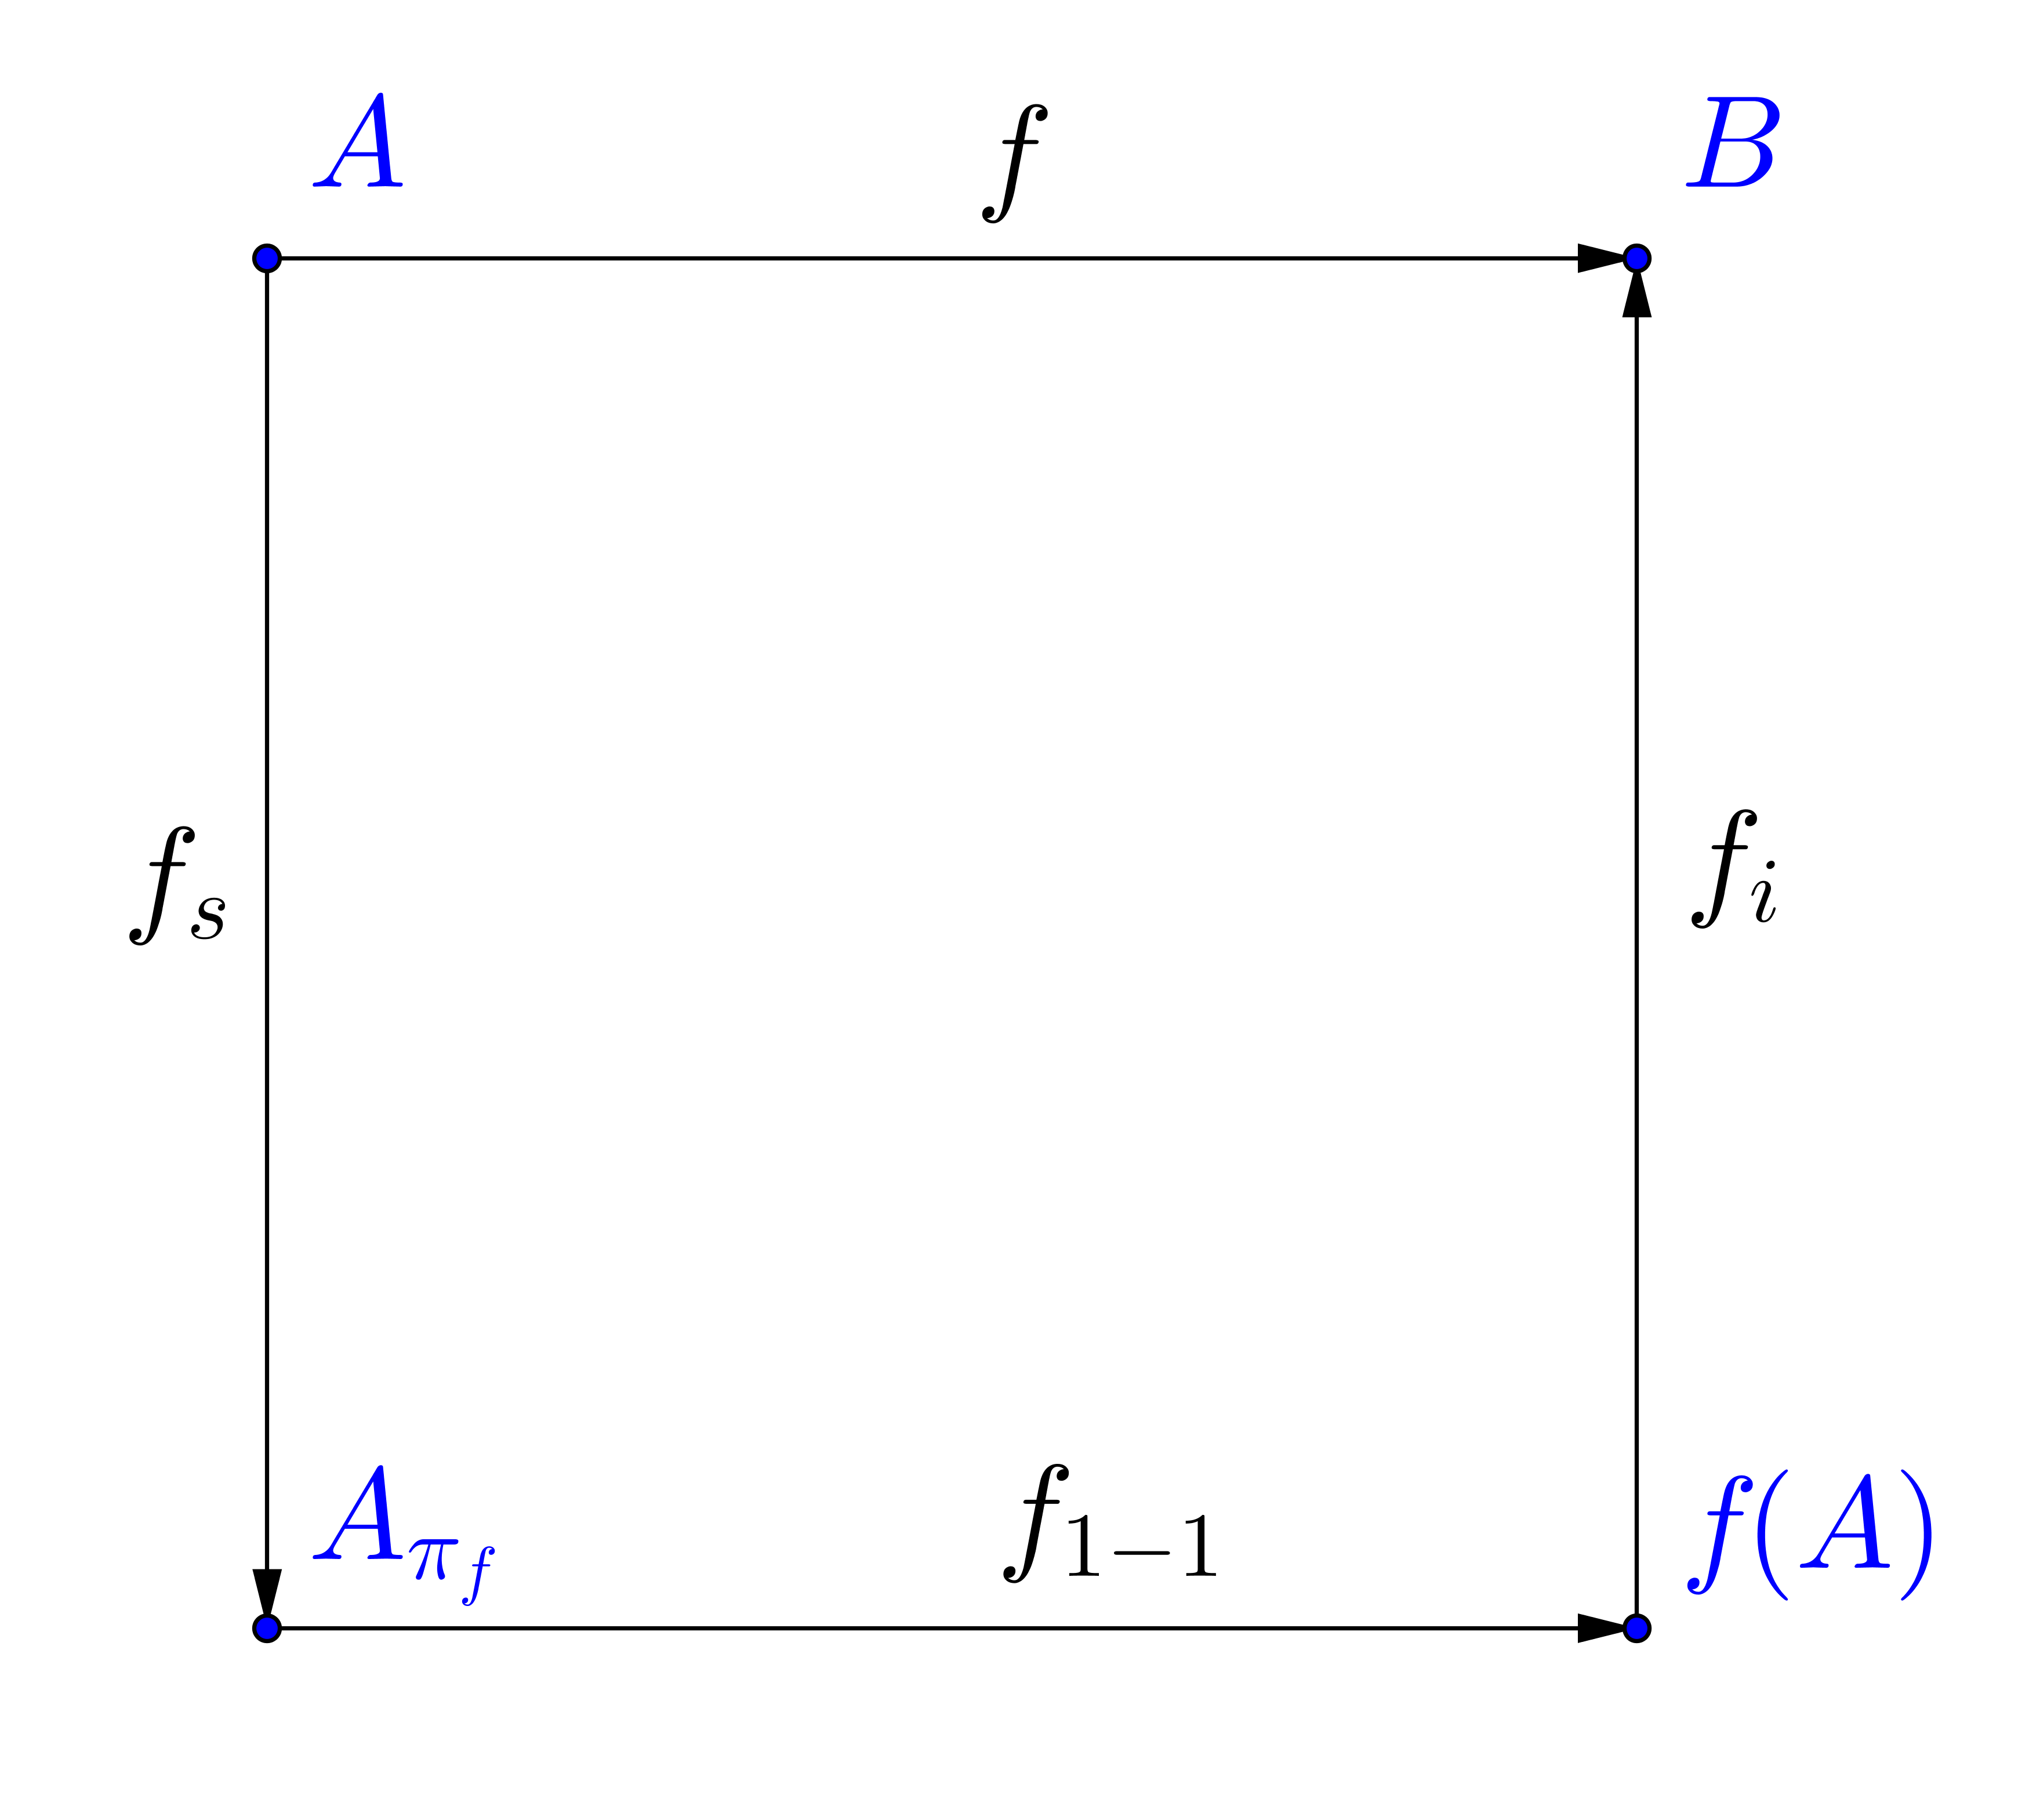
\includegraphics[width=0.6\linewidth]{lect2/InectBiectSuriect.png}
        \caption{Иллюстрация представления отображения $f$ как суперпозиции суръекции, инъекции и биекции. $f_S$ - суръективное отображение, $f_{1-1}$ - биекция, $f_i$ - инъекция}
    \end{center}
\end{figure}
На данном рисунке изображены четыре множества: $A$, $B$, $A_{\pi_f}$~---фактормножество, и $f(A)$. Множество $A$ суръективно отображается в свое фактормножество $A_{\pi_f}$, из-за ядерной эквивалентности отображения $f$, $A_{\pi_f}$ биективно отображается в $f(A)$. В свою очередь $f(A)$ иньективно вкладывается в $B$ как его подмножество.

\section{О декартовом произведении множеств}
Поговорим о декартовом произведении множеств и  том, как его можно представить через другие операции с множествами. Итак, пусть есть множество индексов $\mathfrak{A} = \{\alpha\}$ и соответствующий этому множеству индексов набор множеств $\{A_{\alpha}|\ \alpha \in \mathfrak{A}\}$. Чему тогда равно произведение $\prod_{\alpha \in \mathfrak{A}}A_{\alpha}$? По крайней мере оно не нулевое так как любое декартово произведение произвольного семейства непустых множеств в непустом количестве непусто (об этом свидетельствует теорема выбора). Оказывается, что
\[
\prod_{\alpha \in \mathfrak{A}}A_{\alpha} = \{f|\ f:\ \mathfrak{A}\rightarrow\bigcup_{\alpha \in \mathfrak{A}}A_{\alpha}, \forall\alpha\in\mathfrak{A}: f(\alpha)\in A_{\alpha}\}
\]

Например, пусть 
\[
A_{\alpha} = A_{(x, y)} = \{(x', y')| \rho((x,y), (x',y')) \leq 1\}
\]
Тогда,
\[
\prod_{\alpha \in \mathfrak{A}}A_{\alpha} = \{f| f: R^2 \rightarrow R^2,\ \forall (x,y): \rho((x,y), f((x,y))) \leq 1\}
\]
\end{document} 